\documentclass[12pt]{amsart}
\usepackage[a4paper, margin=2.5cm]{geometry}

%%% Importing packages for colorring and plotting
\usepackage{graphicx}
\usepackage{xcolor}

%%% Creating tables with vertical alignment
\usepackage{float}
\usepackage{makecell}
\usepackage{tabularx}
%%%

%%% Adding references
\usepackage{biblatex}
\addbibresource{references.bib}
%%%

\title{UNICORN Paper Template}
\author{Danfeng Chen}
\date{June 11, 2019} % delete this line to display the current date

%%% BEGIN DOCUMENT
\begin{document}

\maketitle

A major obstacle to the successful identification of genetic risk factors is the availability of large control samples for association studies. Genotyping is often restricted to cases to reduce costs, making analysis impossible without incorporating external controls. While many control resources are available through repositories such as dbGaP, administrative and computational barriers to entry are substantial. Further, controls come from multiple cohorts that may differ in genotyping chip used, genotyping quality and sample ancestry which can lead to batch effects.

The main purpose of this project is to prove the plausibility of harmonizing genotyping data from multiple resources with a thorough and stringent QC pipeline. Our unified QC pipeline ensures reproducibility, extensibility and usability. We also provide a statistical framework to make use of our external controls for genome-wide association test without direct accessing individual-level data. 

\tableofcontents

\section{Harmonizing Genotyping data from multiple sources}

Merging data from multiple genotyping array platforms creates various challenges, which we address with a multi-stage pipeline. We first performed pre-imputation quality control at the cohort and platform levels. We then imputed the platform-level data using the Michigan Imputation Server, merged the results and performed further post-imputation QC. Finally, we used this merged data to identify, remove and re-impute additional poorly performing SNPs on a per-platform basis. The pipeline was implemented in Hail, scalable open source genetics software. This reproducible framework allows additional controls to be incorporated easily, and enables users to run the pipeline on case sets.

\subsection{QC Pipeline}

\begin{figure}
    \centering
    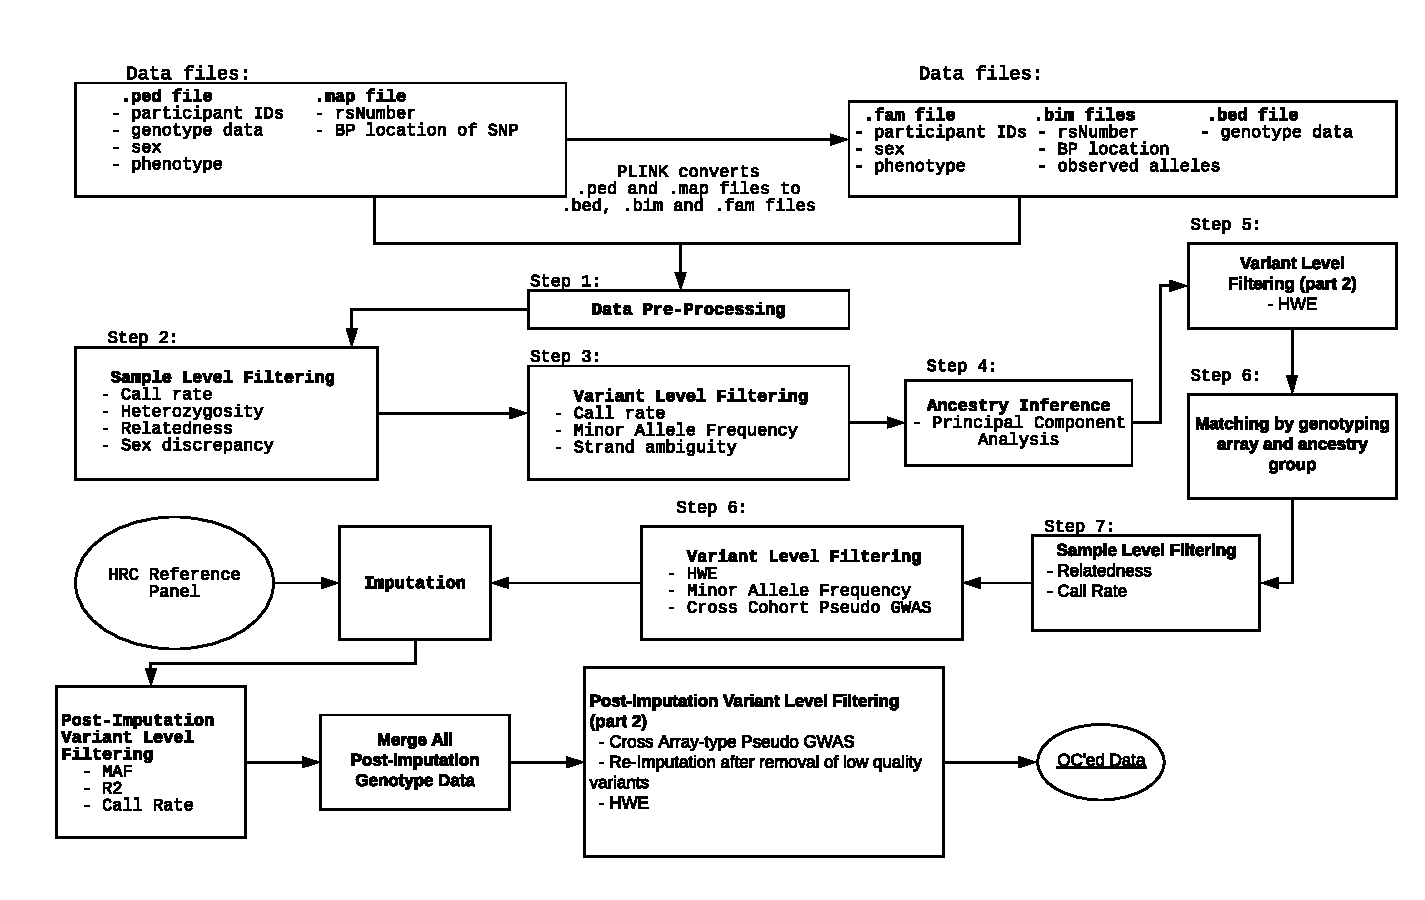
\includegraphics[width=\textwidth]{qc/pipeline.pdf}
    \caption{QC Pipeline}
    \label{fig:qc_pipeline}
\end{figure}


\subsubsection{Data pre-precessing}
All cohorts were lifted over from hg18 to hg19 using liftOver tool. Marker names across all cohorts were made consistent with HRC reference panel based on chromosome, position, and alleles. Indels and missing alleles, duplicated markers, non-matching SNPs were excluded. 

\subsubsection{Cohort-level pre-imputation QC}

\begin{itemize}
\item \emph{Sample QC:} sample with missing rate greater than 2\% or with mismatching sex information between genotypes and provided phenotype information were excluded. Samples with abnormal inbreeding coefficients (3 standard deviation away from its mean) were removed. Related samples (pi-hat $>$ 0.625) were identified and samples from each pair with higher missingness was removed from the data. 
\item \emph{Variant QC:} variant-level missingness was calculated and variants with missing rate $>$ 1\% were excluded. Additionally, all A/T and C/G SNPs were excluded at this point to avoid downstream issues related to strandness. 
\item \emph{Ancestry Inference:}  we built a random forest classifier with the first 6 PCs from 1000 genomes to determine the sub-groups of East Asian ancestry, South Asian ancestry, African ancestry, American ancestry and European ancestry. To further separate population isolates from major European, we build another random forest classifier to determine sub-groups of major European ancestry, Finnish ancestry and Ashkenazi Jewish ancestry with first 4 PCs calculated from a merged set of 1000 genomes European and controls from an Ashkenazi Jewish cohort. We projected each cohort onto the 1000 genome PC spaces, and assigned ancestry-group to samples with RF classifier.  Each sample was assigned to one continental ancestry group. Similar procedure being applied to samples assigned to European ancestry to determine its finer ancestral origin. Within each ancestral group, variants with minor allele frequencies lower than 0.01 or with p-values for Hardy Weinberg Equilibrium test less than $10^{-4}$ were excluded.
\end{itemize}

\subsubsection{Array-level pre-imputation QC}
\begin{itemize}
\item \emph{Matching:} cohorts from same genotyping array and ancestry-group were merged together for downstream analysis.
\item \emph{Sample QC:} sample with missing rate greater than 2\% or related samples with higher missingness was removed.
\item \emph{Variant QC:} within each array group, variants with minor allele frequencies lower than 0.01 or with p-values for Hardy Weinberg Equilibrium test less than $10^{-4}$ were excluded. To further identify variants susceptible to batch effects, a pseudo GWAS comparison tagging array samples as cases and 1000 Genomes samples as controls were performed,  and variants with p-values less than $10^{-4}$ were excluded. Moreover, another type of pseudo GWAS comparisons tagging samples from one cohort as cases and samples from other cohorts as controls were carried out, and variants with p-values less than $10^{-4}$ were excluded. For pseudo GWAS comparison, first 20 PCs were included as covariates to control population stratification.
\end{itemize}

\subsubsection{Imputation}
We imputed each stratum separated based on 1000 genomes reference panel using Michigan Imputation server. 

\subsubsection{Post-imputation QC}
Using all variants for downstream analysis without a careful quality control will lead to a severe batch effects as certain regions of the genome are different to impute due to the low coverage in the reference panel or high recombination rate. Moreover, when considering the issue of batch effects will become more severe when considering using merged imputed genotypes. Different genotyping arrays have different backbones will result in differences in imputation quality, which becomes the source of batch effects. 

Many post-imputation QC metrics were proposed to measure the variant imputation quality. The most widely used post-imputation variant quality control measures for Rsq and AvgCall. Rsq is defined to be the estimated squared correlation between imputed genotypes and true, unobserved genotypes. AvgCall is average probability (certainty) of observing the most likely allele for each haplotype. There are some other post-impuation QC metrics, such as EmpRsq and CallRate, are also used to measure the imputation quality. EmpRsq is correlation between the true genotyped values and the imputed dosages that were calculated by hiding all known genotyped for the given SNP; it is only defined for typed variants. In terms of call rate, we define any genotype with a posterior probability $\geq$ certain threshold (0.9) was defined as called, and genotypes at SNPs with a maximum posterior probability below this threshold were classified as missing; defined for all variants. There are no consensus about which QC metrics work best under which scenario. Different imputation tools report different quality measures. A more direct way of measuring batch effects is by pseudo GWAS. For each genotyping array, samples that were genotyped on it were coded as cases and samples that were genotyped on other arrays were coded as controls to make a pseudo-case control comparison. Any variants that are reported to be significant are considered to be susceptible to batch effects. We also applied minor allele frequencies filter as the imputation quality drops down as allele frequencies decreases. The detailed pipeline goes as follows.

\begin{itemize}
\item \emph{QC each array stratum: } After imputation, 46.8M variants had been imputed in each array stratum. Variants with minor allele frequencies $<$ 0.01 or out of Hardy-Weinberg Equilibrium (p $<$ $10^{-4}$) or with an imputation info score $<$ 0.8 were removed from the data.
\item \emph{Inner-join: } a master imputed genotype data were generated through an inner join across all stratum together.
\item \emph{Cross-array comparison: }for each genotyping array, samples that were genotyped on it were coded as cases and samples that were genotyped on other arrays were coded as controls to make a pseudo-case control comparison. To run the association testing, we added first 20 PCs as covariates and drop variants with p-values $<$ $10^{-5}$.
\item \emph{Re-imputation:} We remove variants with empRsq $<$ 0.6 from the typed data, and re-impute them back so as to increase the number of SNPs as well as to improve the quality. The detailed discussion for re-imputation could be found in latter paragragh.
\end{itemize}

\subsection{Control Repository Summary}


\subsubsection{Input Data Summary}
Till this end, we have aggregated 27517 self-reported European-descent control samples obtained from 16 collections within dbGaP data repository. These were genotyped on a plethora of technologies including Illumina and Affymetrix arrays. 

\begin{table}[H]
\begin{tabular}{llllll}
\hline
Genotyping Array & nSamples & nSNPs & nCohorts & Ancestry & Country \\
\hline
Affy6                 & 4504   & 907K  & 3  & European & USA \\
Axiom                 & 10000  & 636K  & 1  &
European & USA \\
Human300             & 219    & 300K  & 1  &
European & USA \\
Human550              & 5559   & 550K  & 5  & European & USA \\
Human610              & 4672   & 610K  & 4  & European & USA \\
Human660              & 2563   & 660K  & 2  & European & USA \\
\hline
\end{tabular}
\end{table}

\subsubsection{Pre-imputation QC}
After pre-imputation QC, a total of 22510 samples retained. Here is a summary of samples by genotyping array. Among 5007 samples that are removed during the QC, 1570 are with less than 0.8 probability of being classified into European mainland Ancestry using random forest classifier. 579 samples are filtered due to high sample missing rate. The rest 2858 samples are filtered out because of relatedness or abnormal inbreeding coefficient. 

For pre-imputation variant QC, in additional to ordinary QC filters such as missing rate, minor allele frequencies and Hardy Weinberg Equilibrium, pseudo GWAS comparing controls against controls and comparing controls against 1000 Genomes European samples are the essential step to identify variants susceptible to batch effects. About 500 variants on average are filtered out in this step for each genotyping platform.

\begin{table}[H]
\begin{tabular}{lll}
\hline
Genotyping Array & nSamples Retained & nVariants Retained \\
\hline
Affy6                 & 2936  & 573K \\
Axiom                 & 9080  & 561K \\
Human300              & 197   & 299K \\
Human550              & 4449  & 460K \\
Human610              & 3604  & 501K \\
Human660              & 2244  & 506K \\
\hline
\end{tabular}
\end{table}

\subsubsection{Imputation and Post-imputation QC} 
After imputation and post-imputation QC, we get 22510 samples and 5524462 variants. Figure 2 provides an overview of post-imputation control repository. 

\begin{figure}[H]
    \centering
    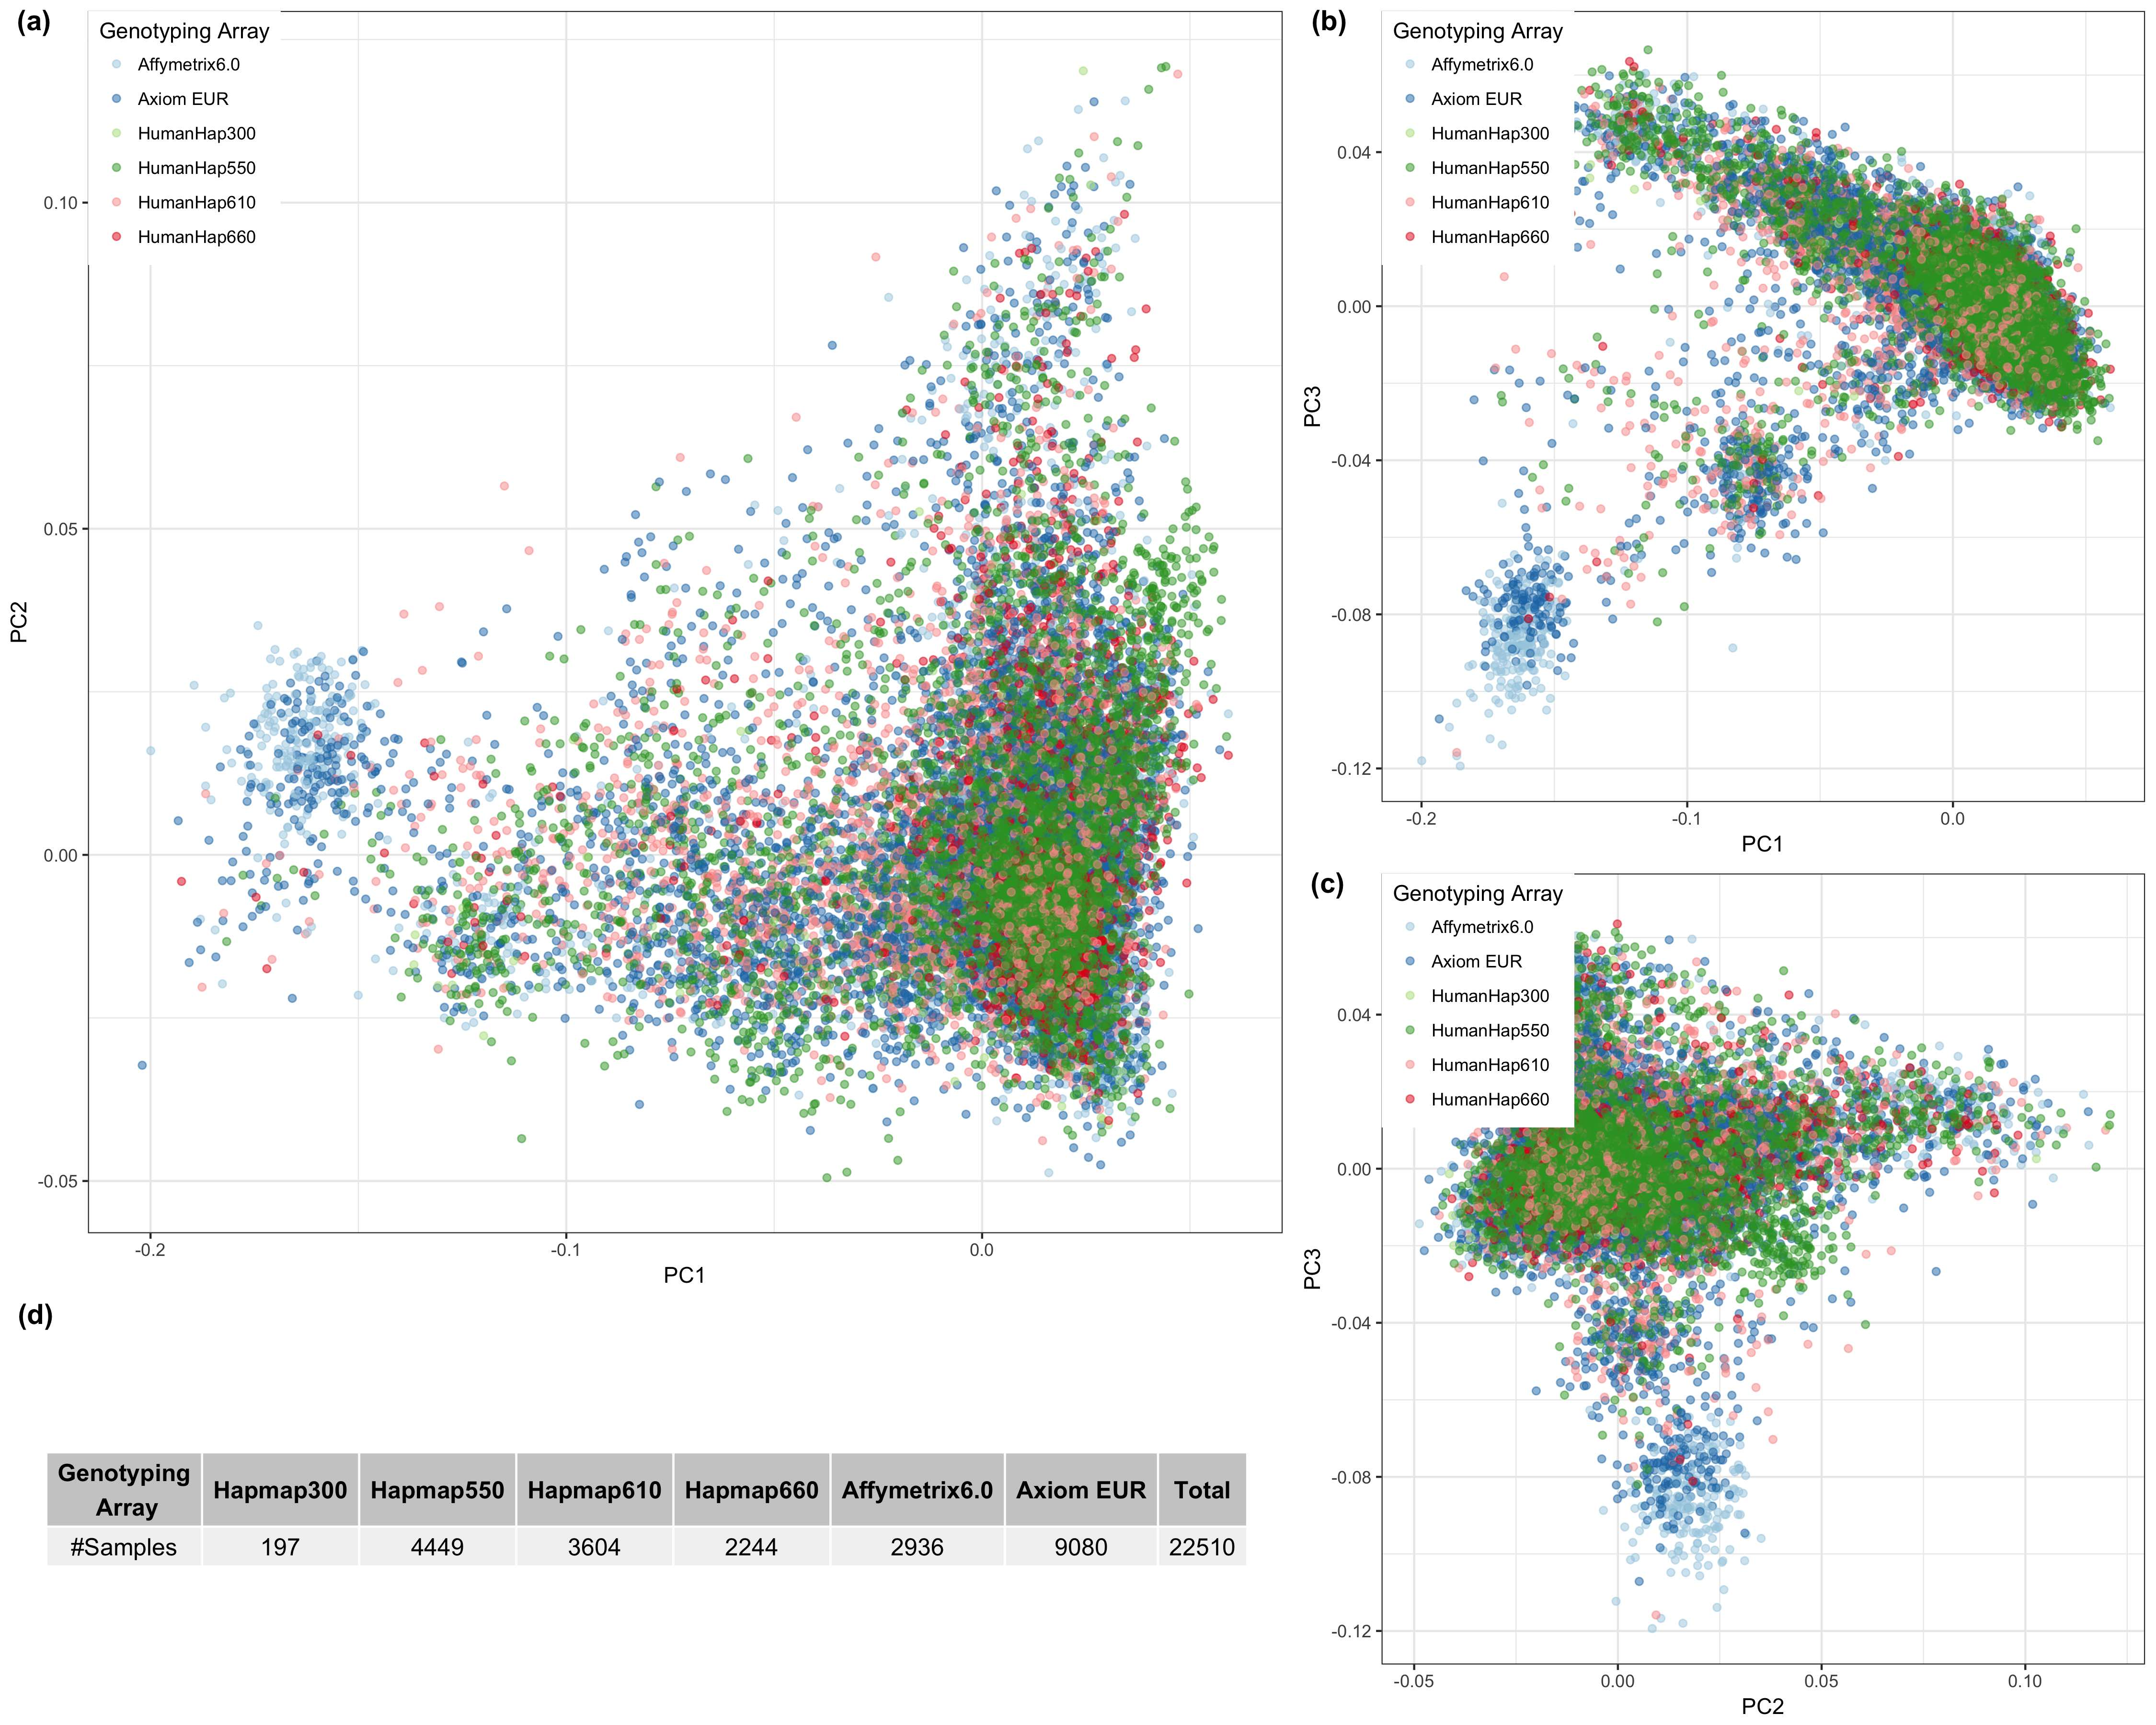
\includegraphics[width=\textwidth]{qc/contRepoPCA.jpg}
    \caption{Control Repository Overview}
    \label{fig:cont_repo}
\end{figure}

\subsection{Performance Evaluation}
We used Crohn's disease genetics data from IBD Genetics Consortium to evaluate the usability of UNICORN controls and the performance of quality control pipeline. First of all, we applied the same pre-imputation quality control pipeline to Crohn's disease data. The cleaned data was imputed against 1000 genomes reference panel. We then removed typed variants with empRsq $<$ 0.6 and re-did imputation. Then, we applied post-imputation QC metrics including MAF $>$ 0.01, Rsq $>$ 0.8 and p-values for pseudo GWAS comparison $> 1e-5$ were applied. GWAS comparing cases from Crohn's genetics data against aggregated UNICORN controls was carried out. GWAS comparing Crohn's cases against Crohn's controls was also performed to provide a reference group. 

First of all, we notice that removing typed variants with low empRsq and re-imputation is one of the essential steps to avoid batch effects. To demonstrate that, we skipped the re-imputation step and generated the GWAS result comparing Crohn's cases against UNICORN controls. We then randomly zoomed-into several regions of different chromosomes. From figure 3, we can observe a co-location of sites that are significant in pseudo-GWAS and sites with low EmpRsq score. 

\begin{figure}[H]
    \centering
    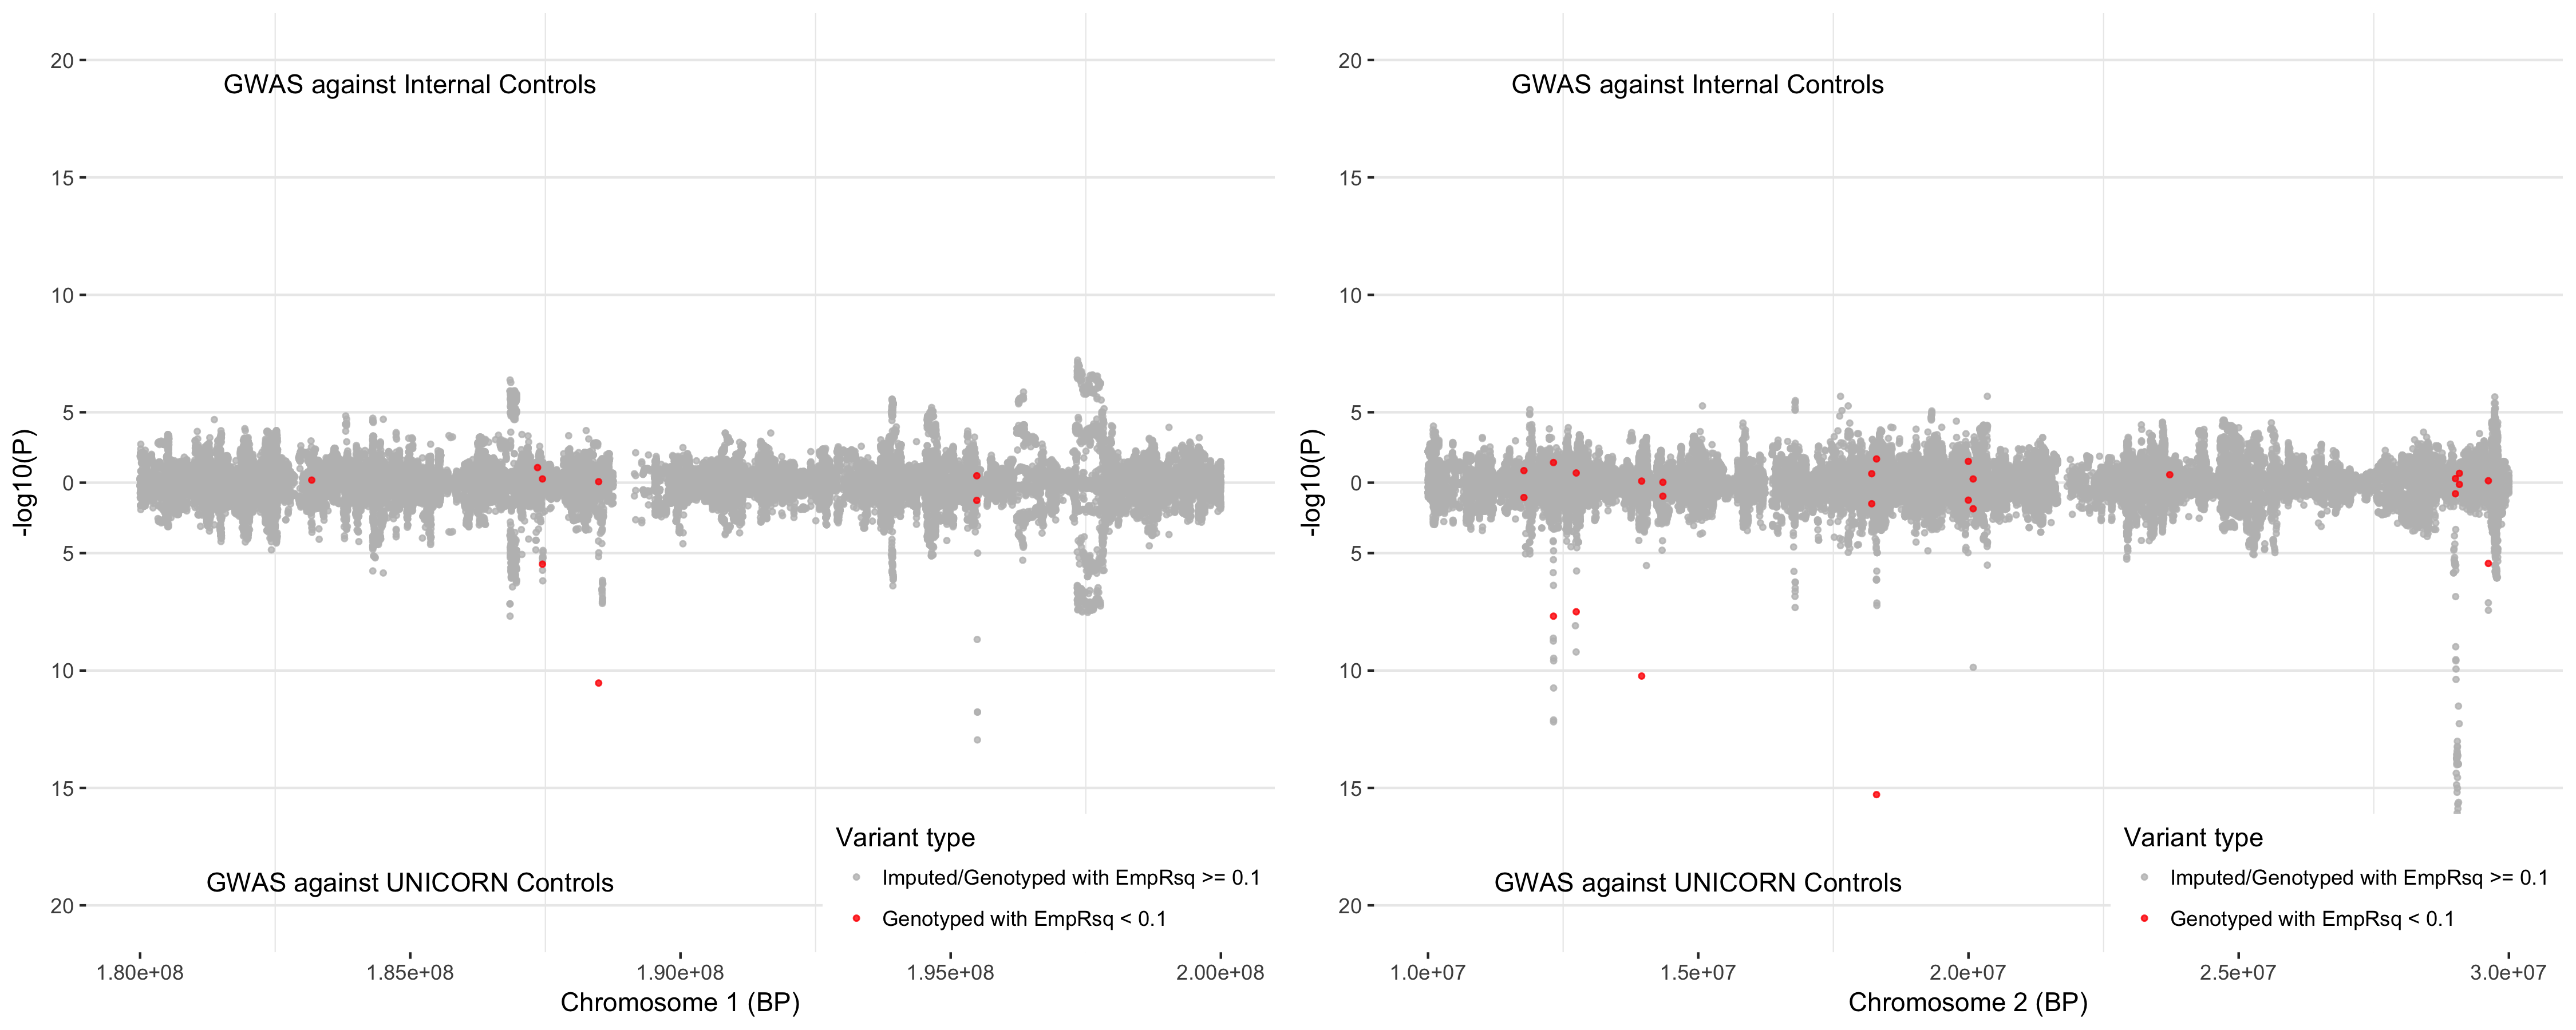
\includegraphics[width=\textwidth]{qc/empRsq.png}
    \caption{Co-localization of batch effects and low empRsq}
    \label{fig:emp_rsq}
\end{figure}

Secondly, the correlation between different QC metrics Rsq, AvgCall and CallRate for same locus are pretty high, suggesting the performance of different QC metrics are similar. Therefore, in our pipeline, we only drop the AvgCall and CallRate as application of other filters could be duplicated. Meanwhile, Rsq/EmpRsq filter and pseudo-GWAS filter are complementary. Finally, the figure 4 shows GWAS against UNICORN controls and internal controls with meta-analysis p-values in light grey. We can see that there is a good concordance between GWAS results calculated from UNICORN controls and standard GWAS association statistics at the broad level. Significant Crohn's disease loci were also reported through comparing against UNICORN controls. We randomly zoomed-into 2 regions of the chromosome, we can see that even at a finer scale, the concordance is pretty well. Meanwhile, the zoom-in at chromosome 5 also shows that using external controls could provide a boost in power.

\begin{figure}[H]
    \centering
    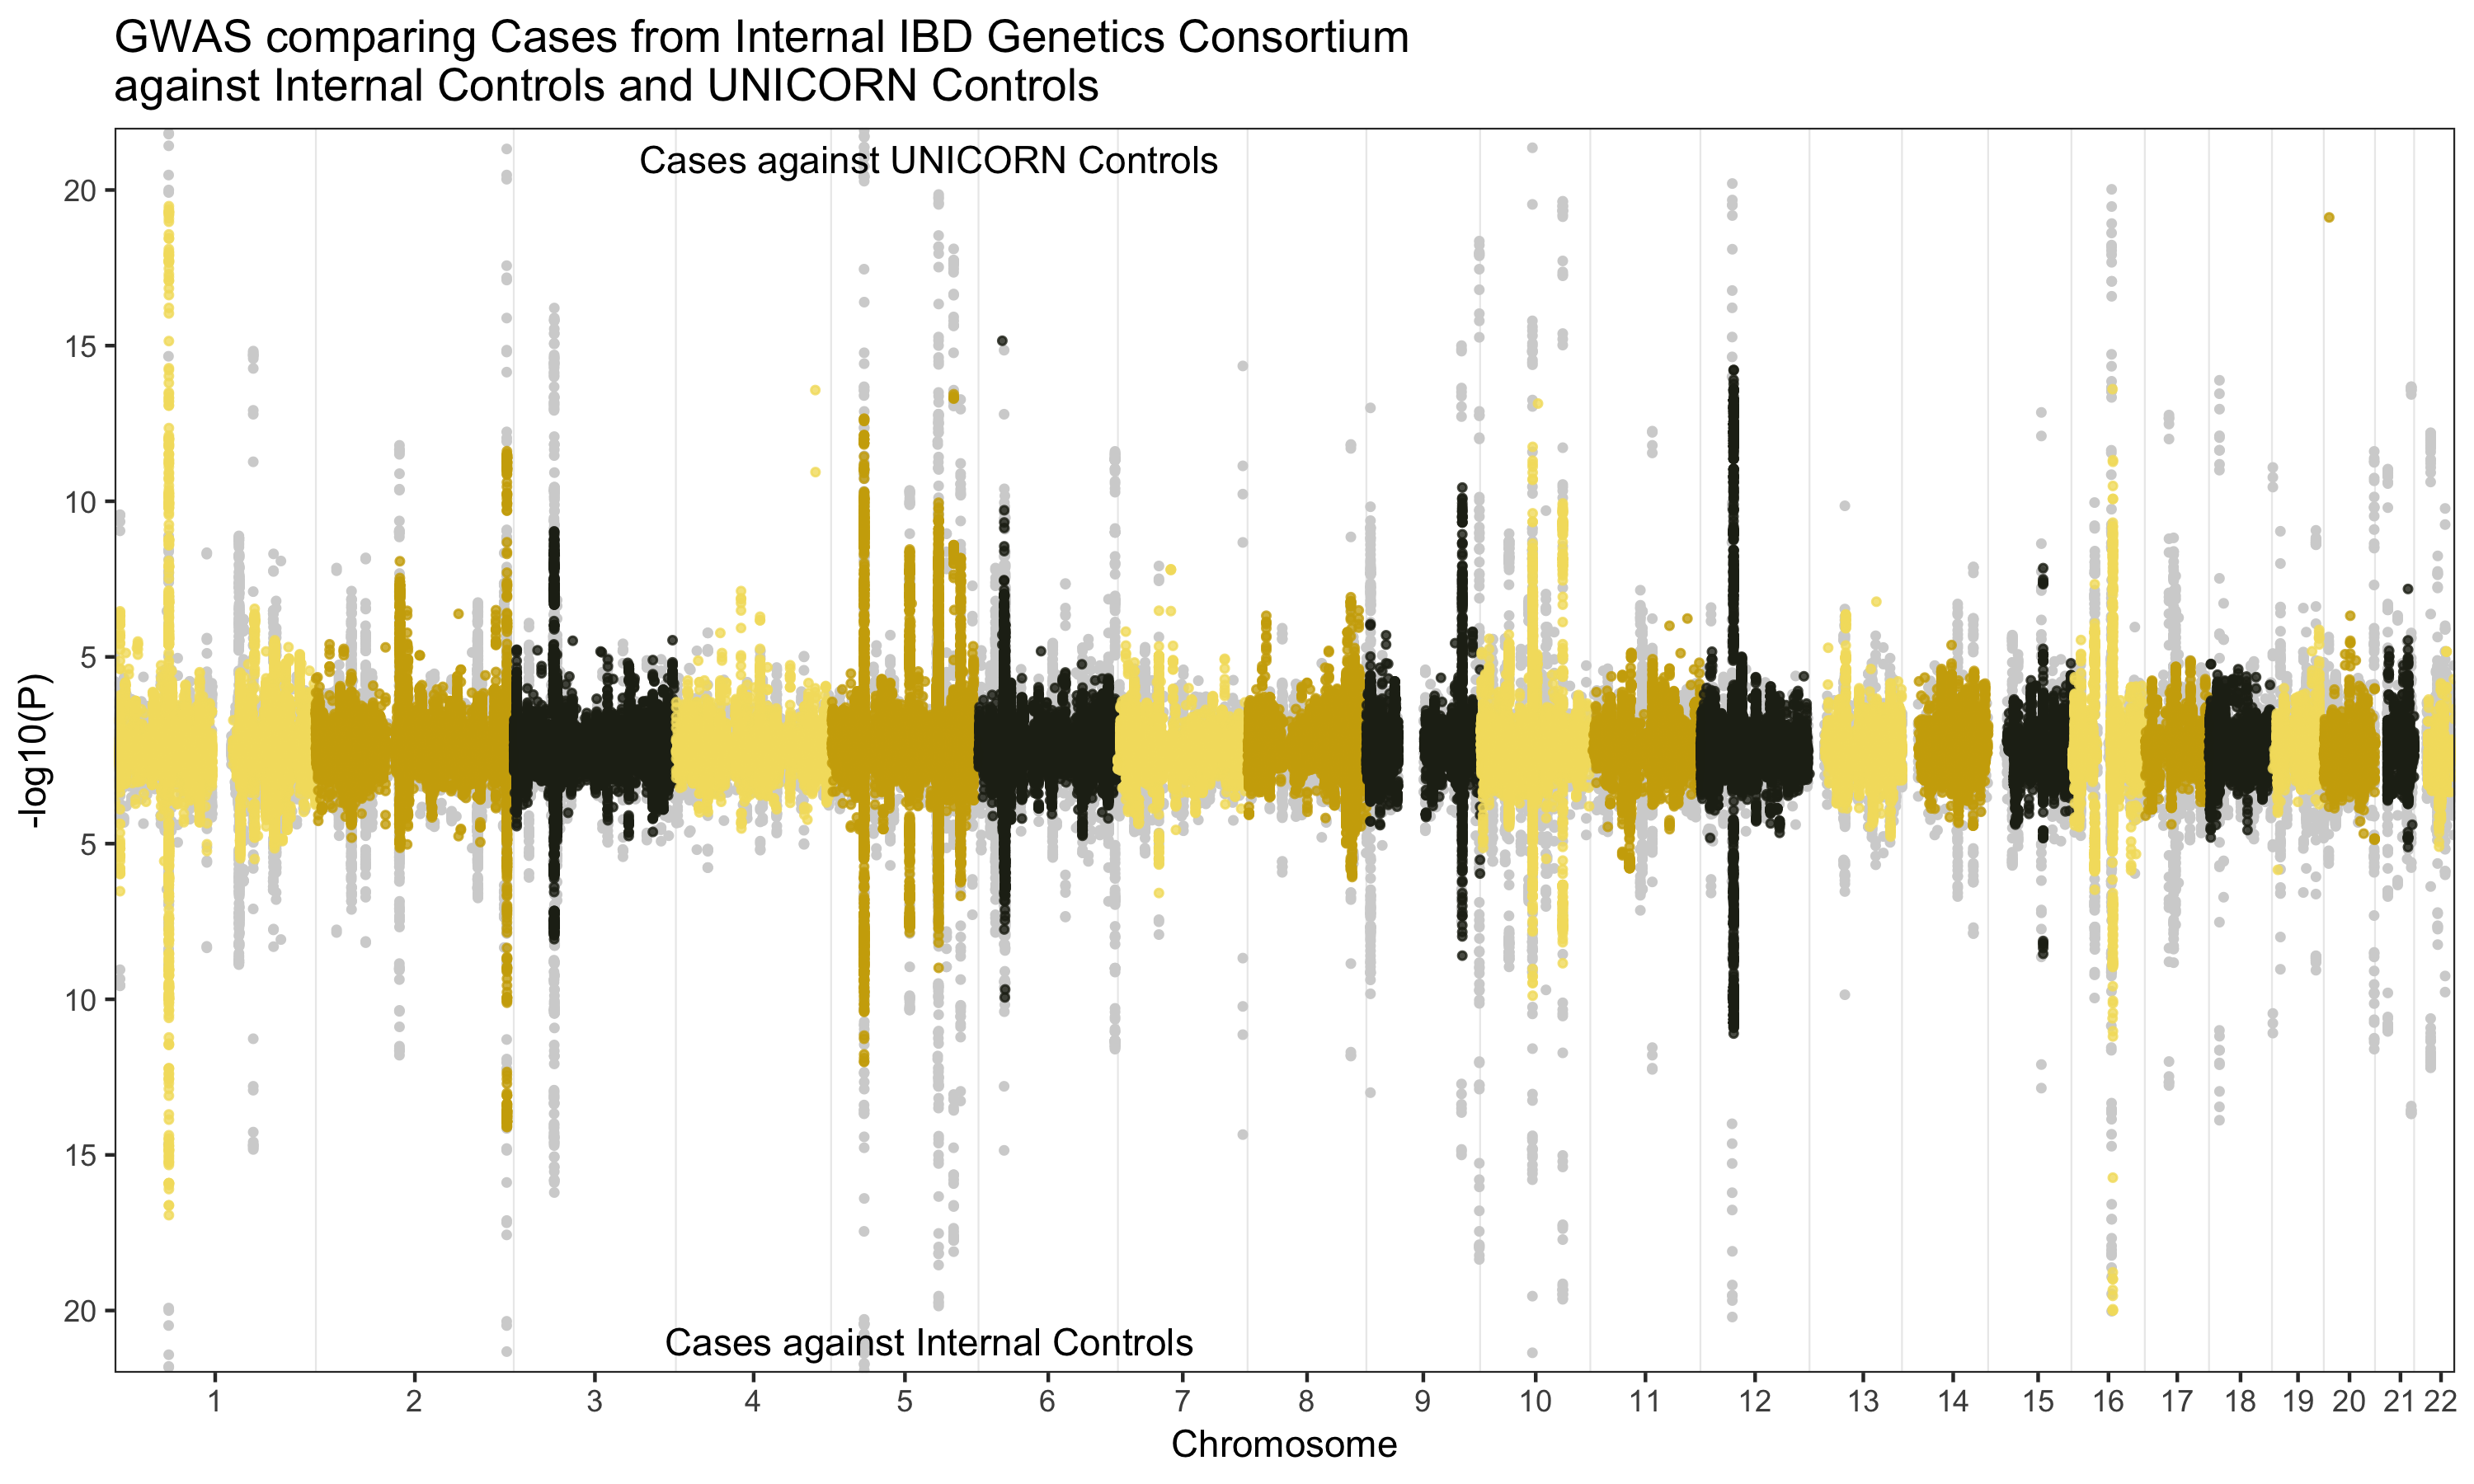
\includegraphics[width=\textwidth]{qc/manhattan.png}
    \caption{GWAS against UNICORN controls}
    \label{fig:gwas}
\end{figure}
\begin{figure}[H]
    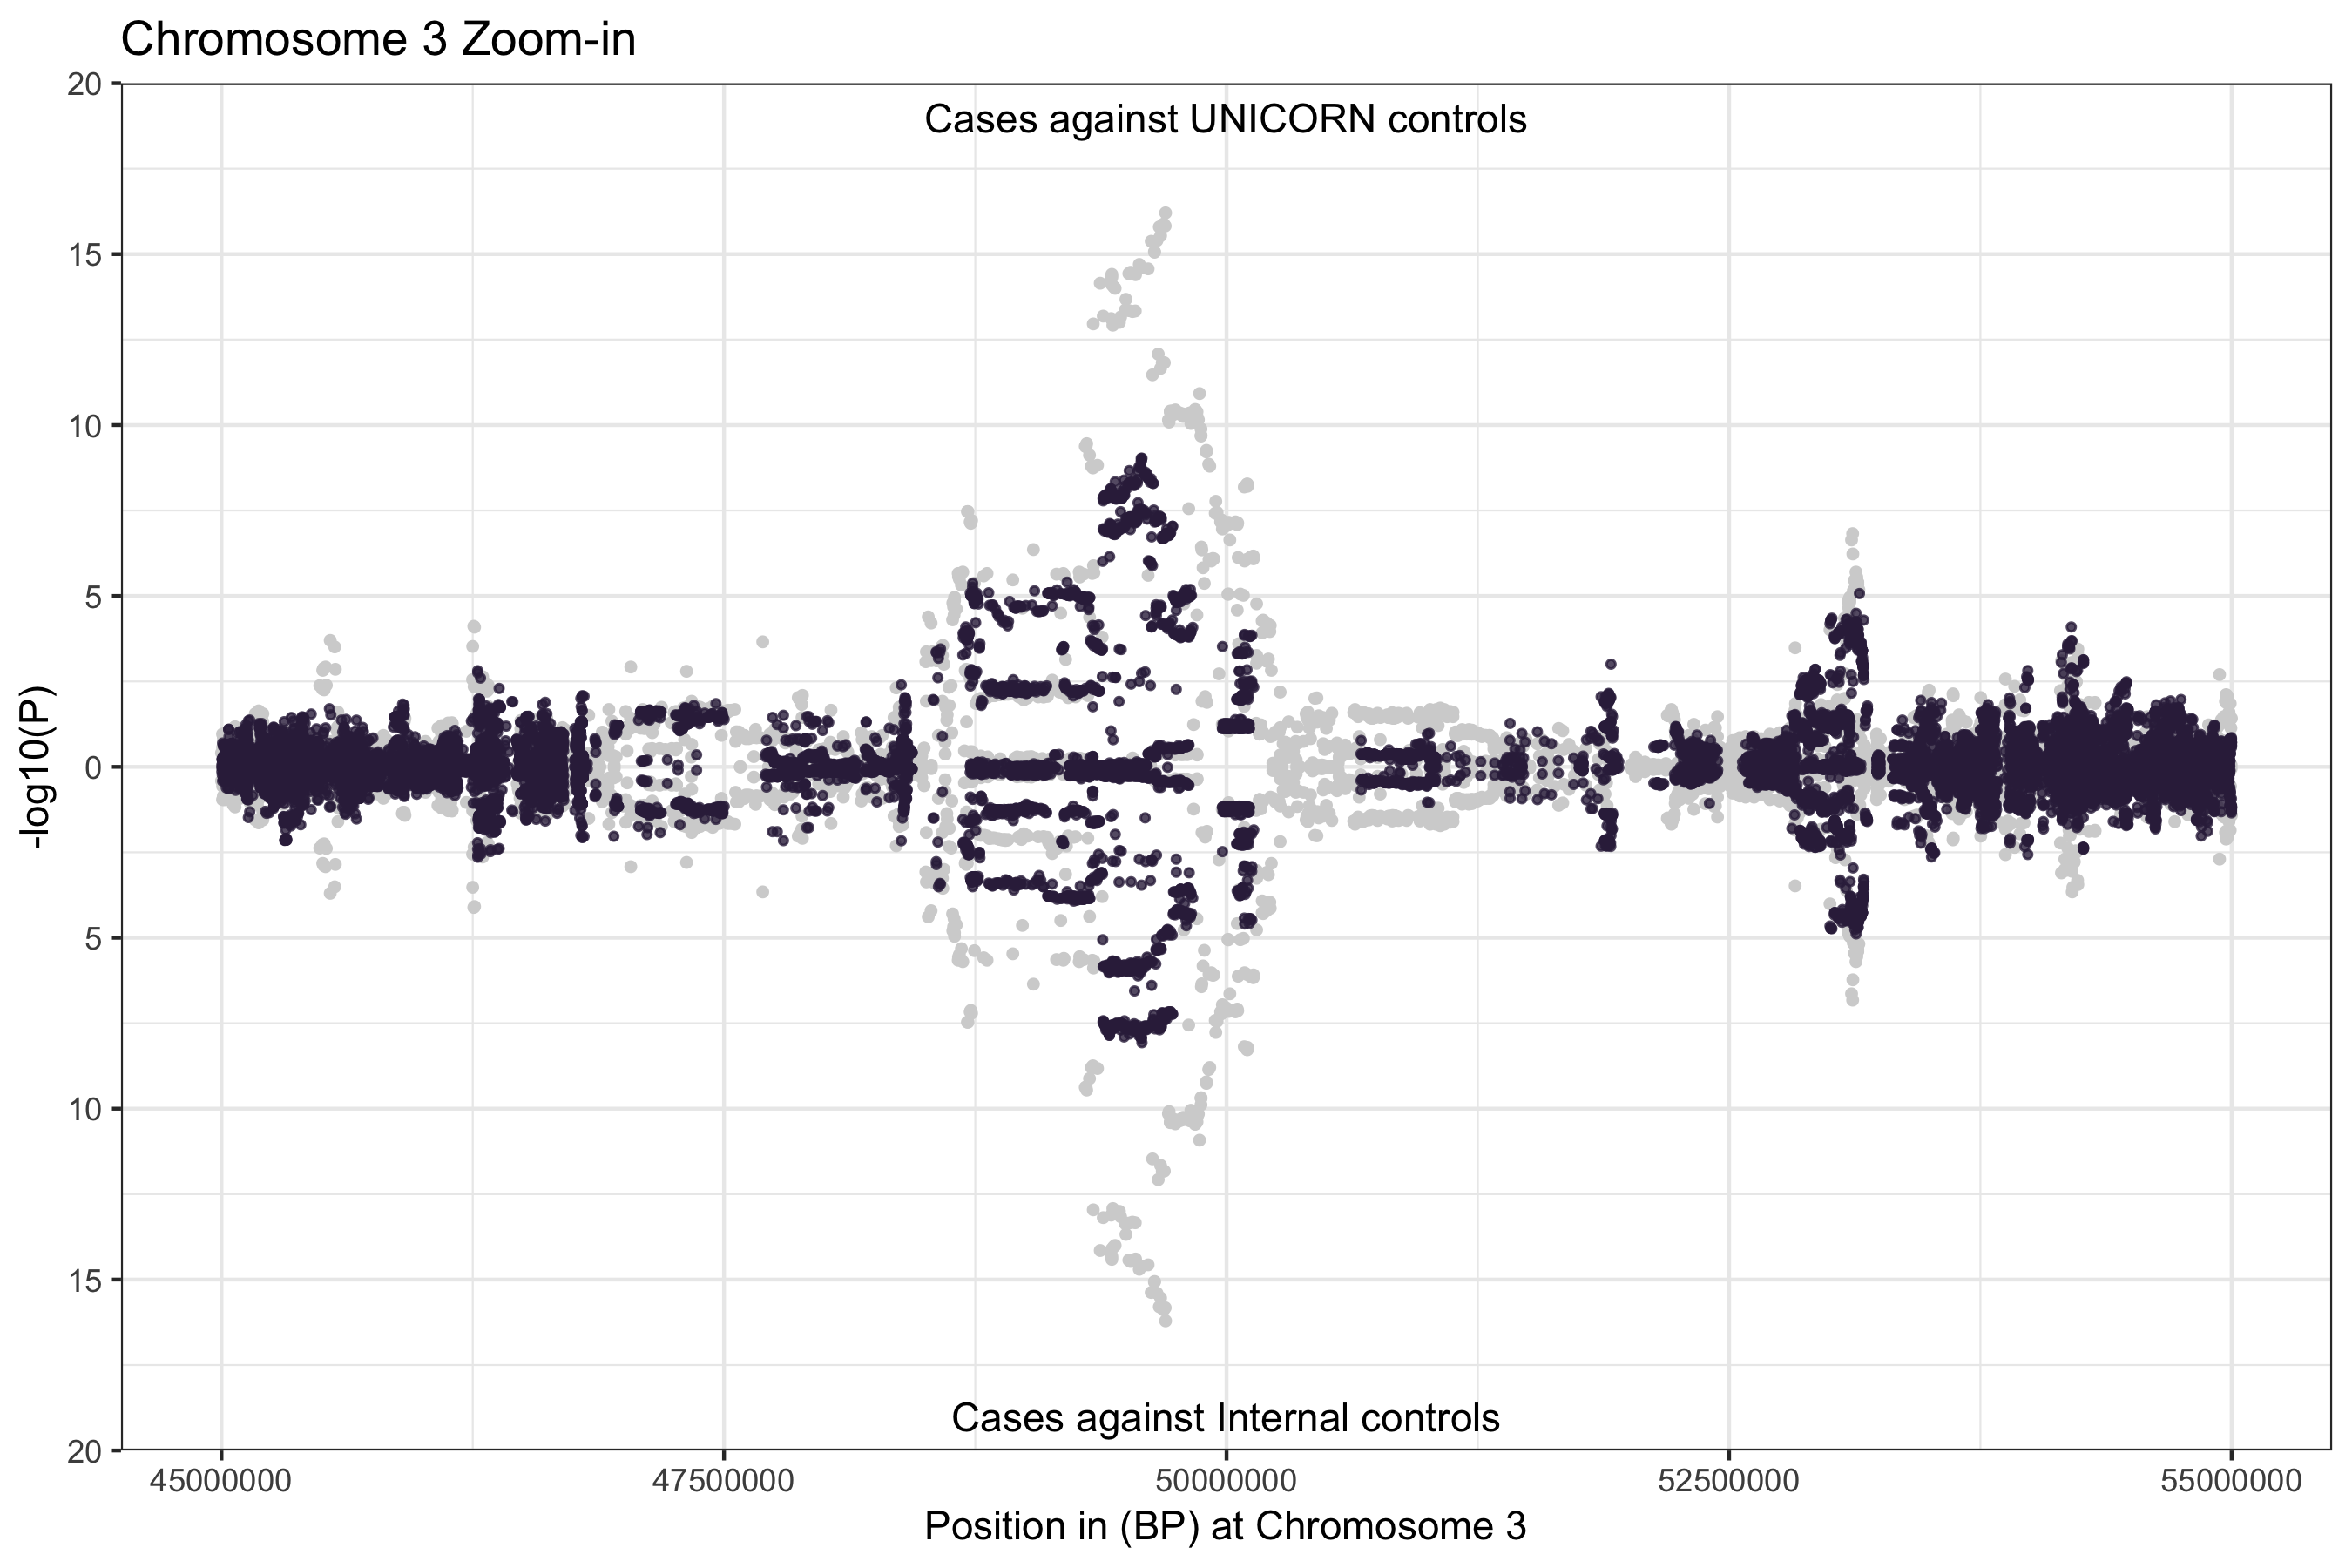
\includegraphics[width=0.48\textwidth]{qc/manhattan_zoom_in1.png}
    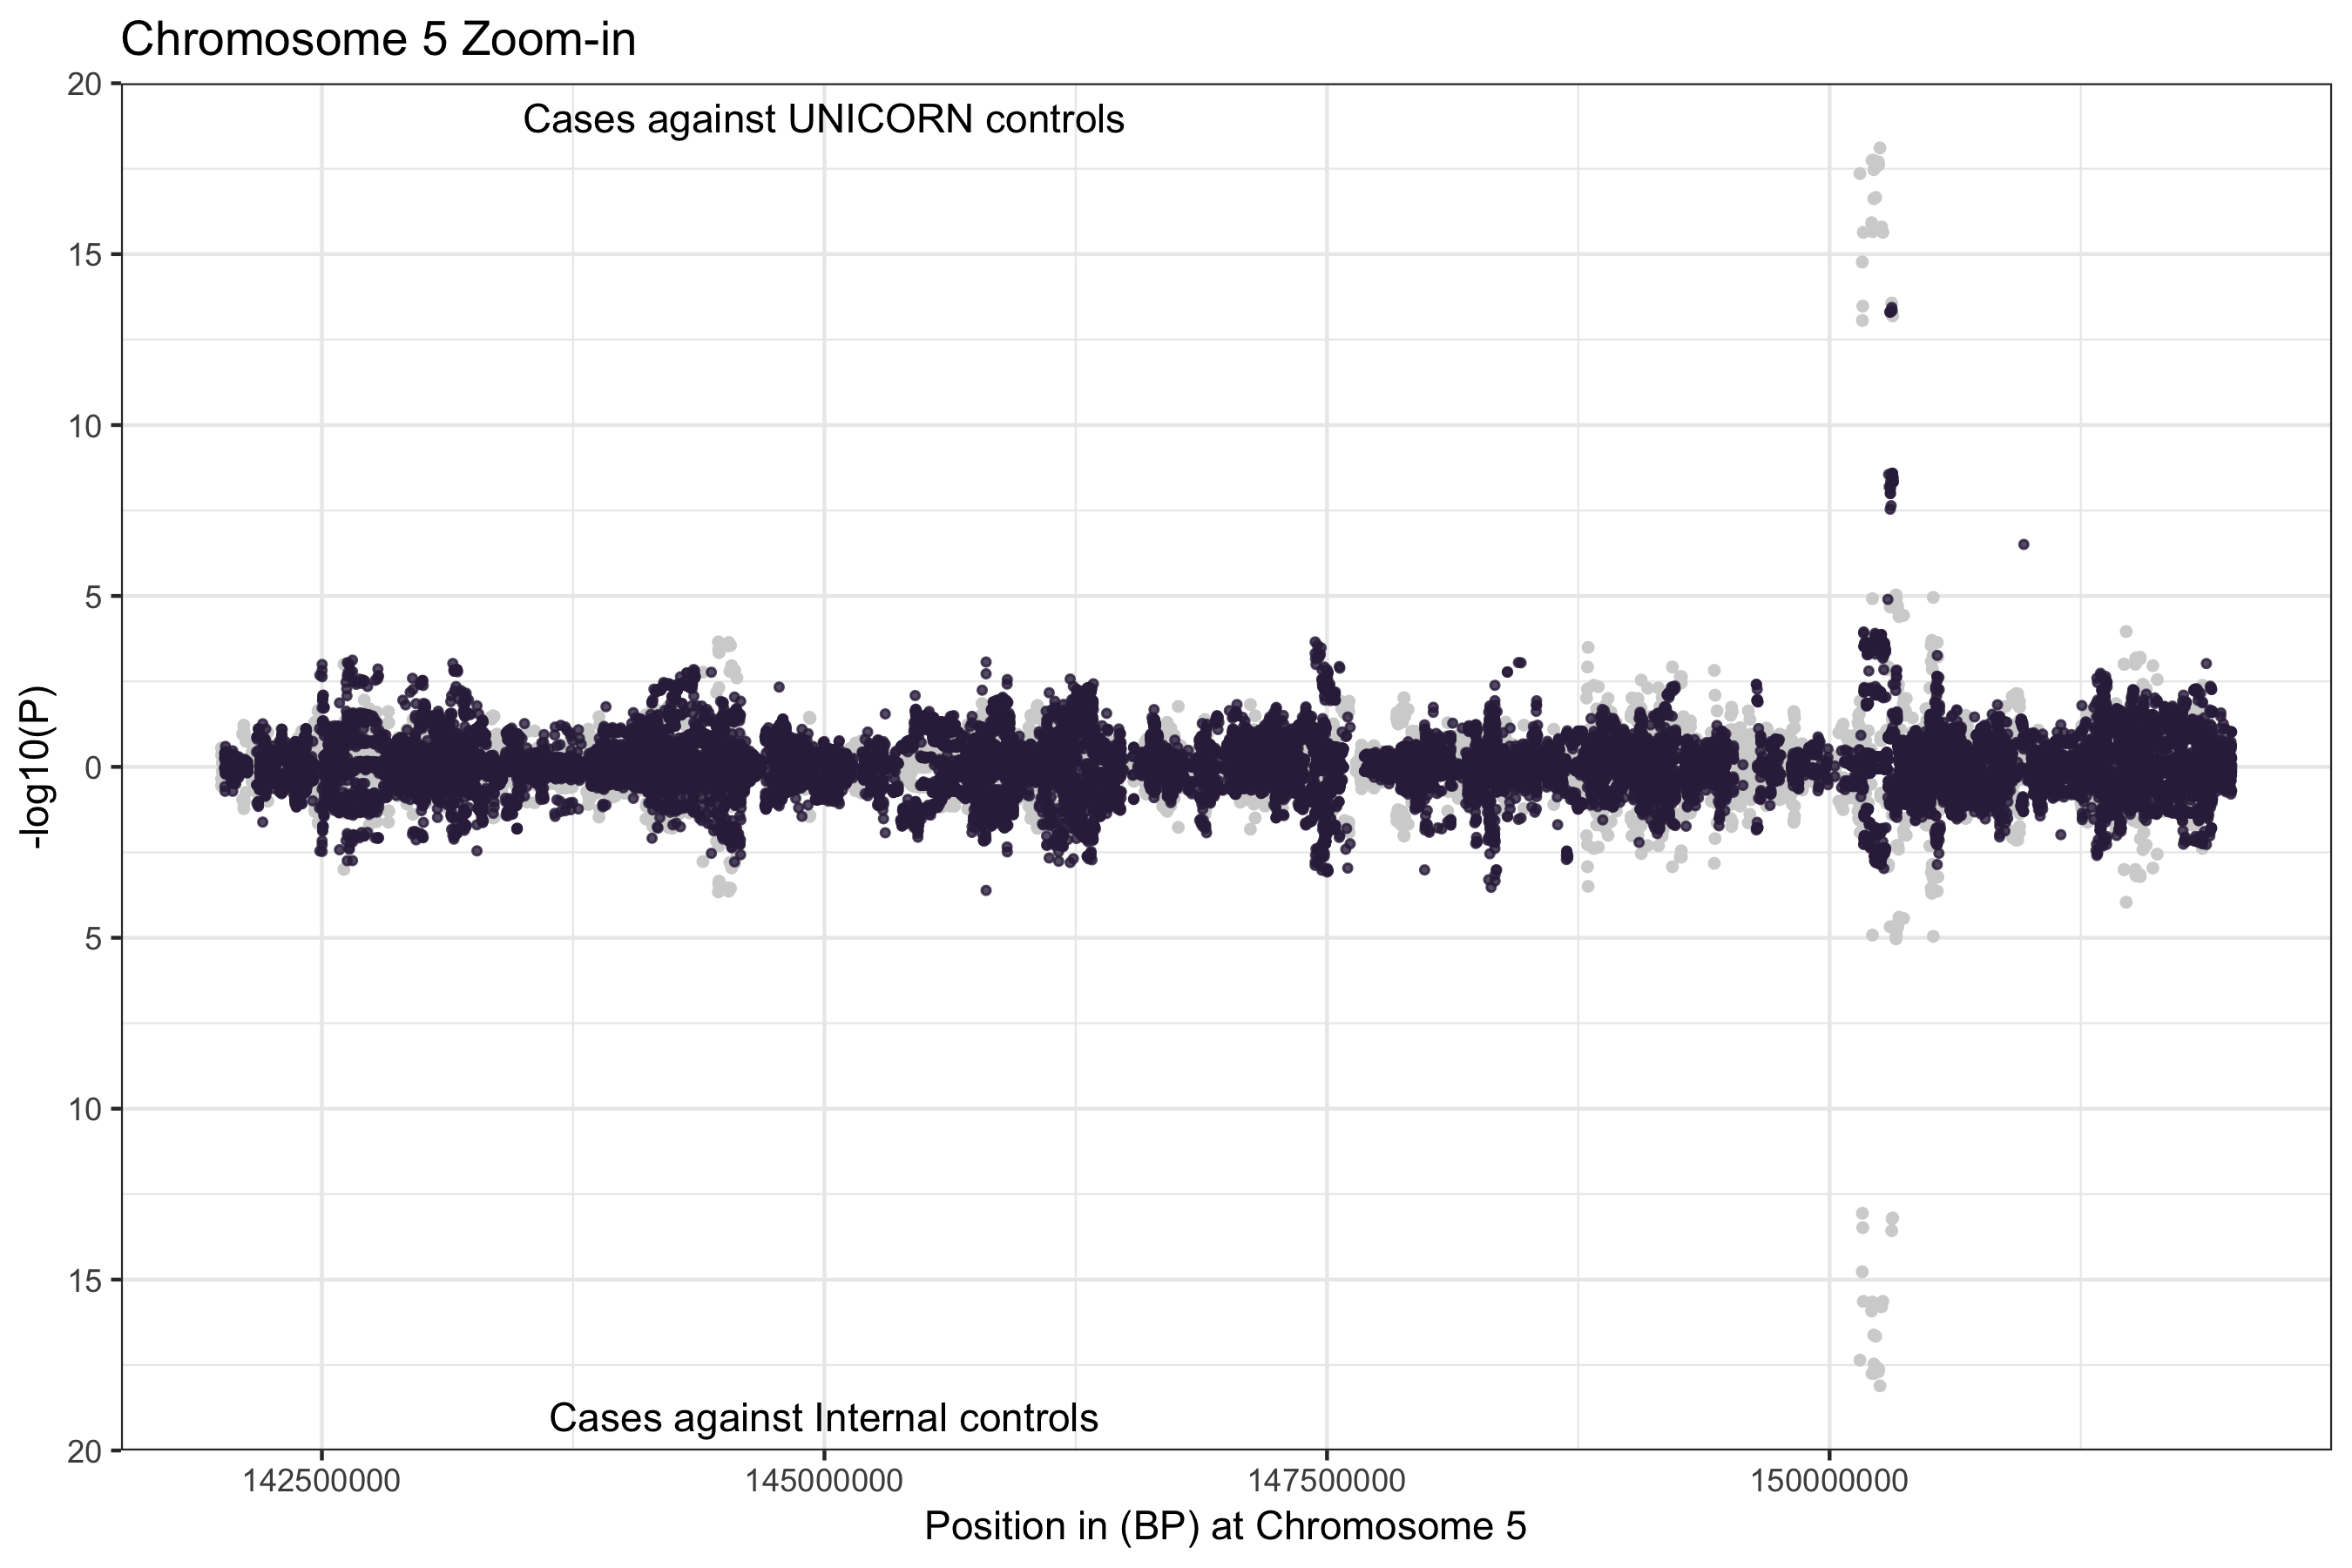
\includegraphics[width=0.48\textwidth]{qc/manhattan_zoom_in2.png}
    \caption{GWAS against UNICORN controls}
    \label{fig:gwas}
\end{figure}

To further examine whether using external UNICORN controls can provide a boost in power while still yield low false positive rate under null, we compared the p-values from different controls, restricting to variants that are significant and non-significant in meta-analysis. The plot on the left demonstrates that under the null, using UNICORN controls doesn't improve the false positive rate. The plot on the right shows that the power to detect genetic signal increases with UNICORN controls.


\begin{figure}[H]
    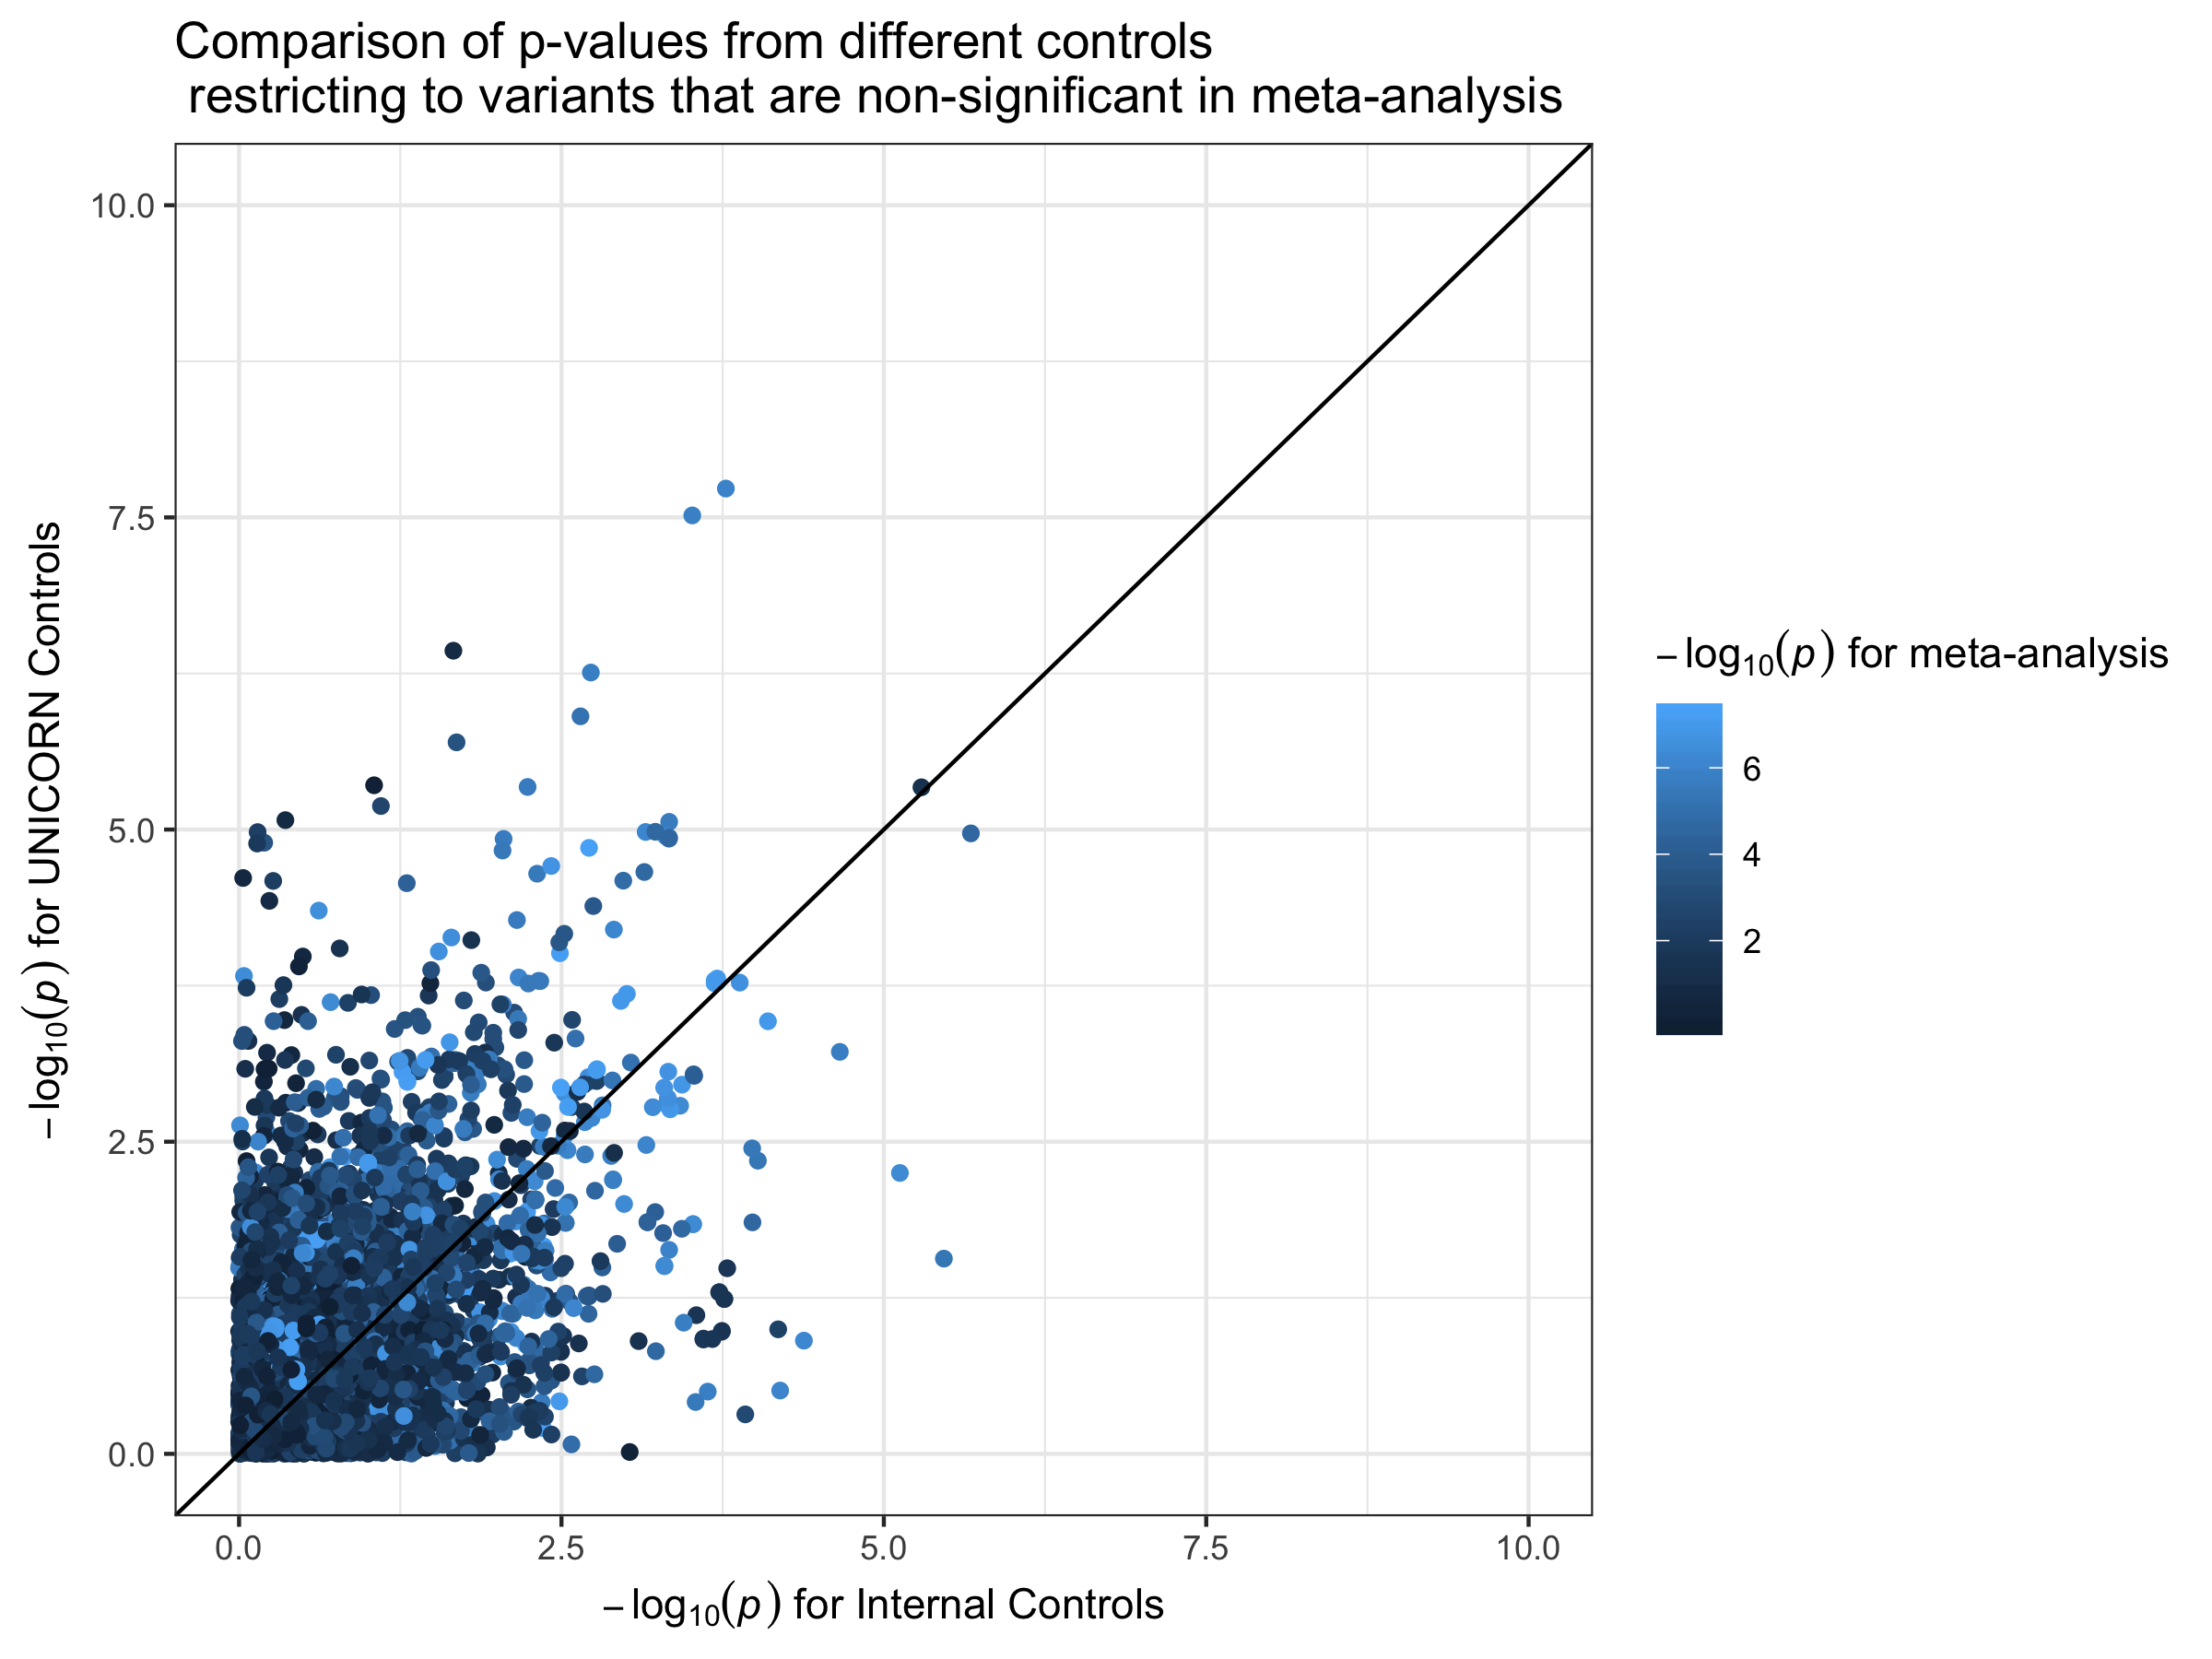
\includegraphics[width=0.49\textwidth]{qc/pvalues_non-significant.png}
    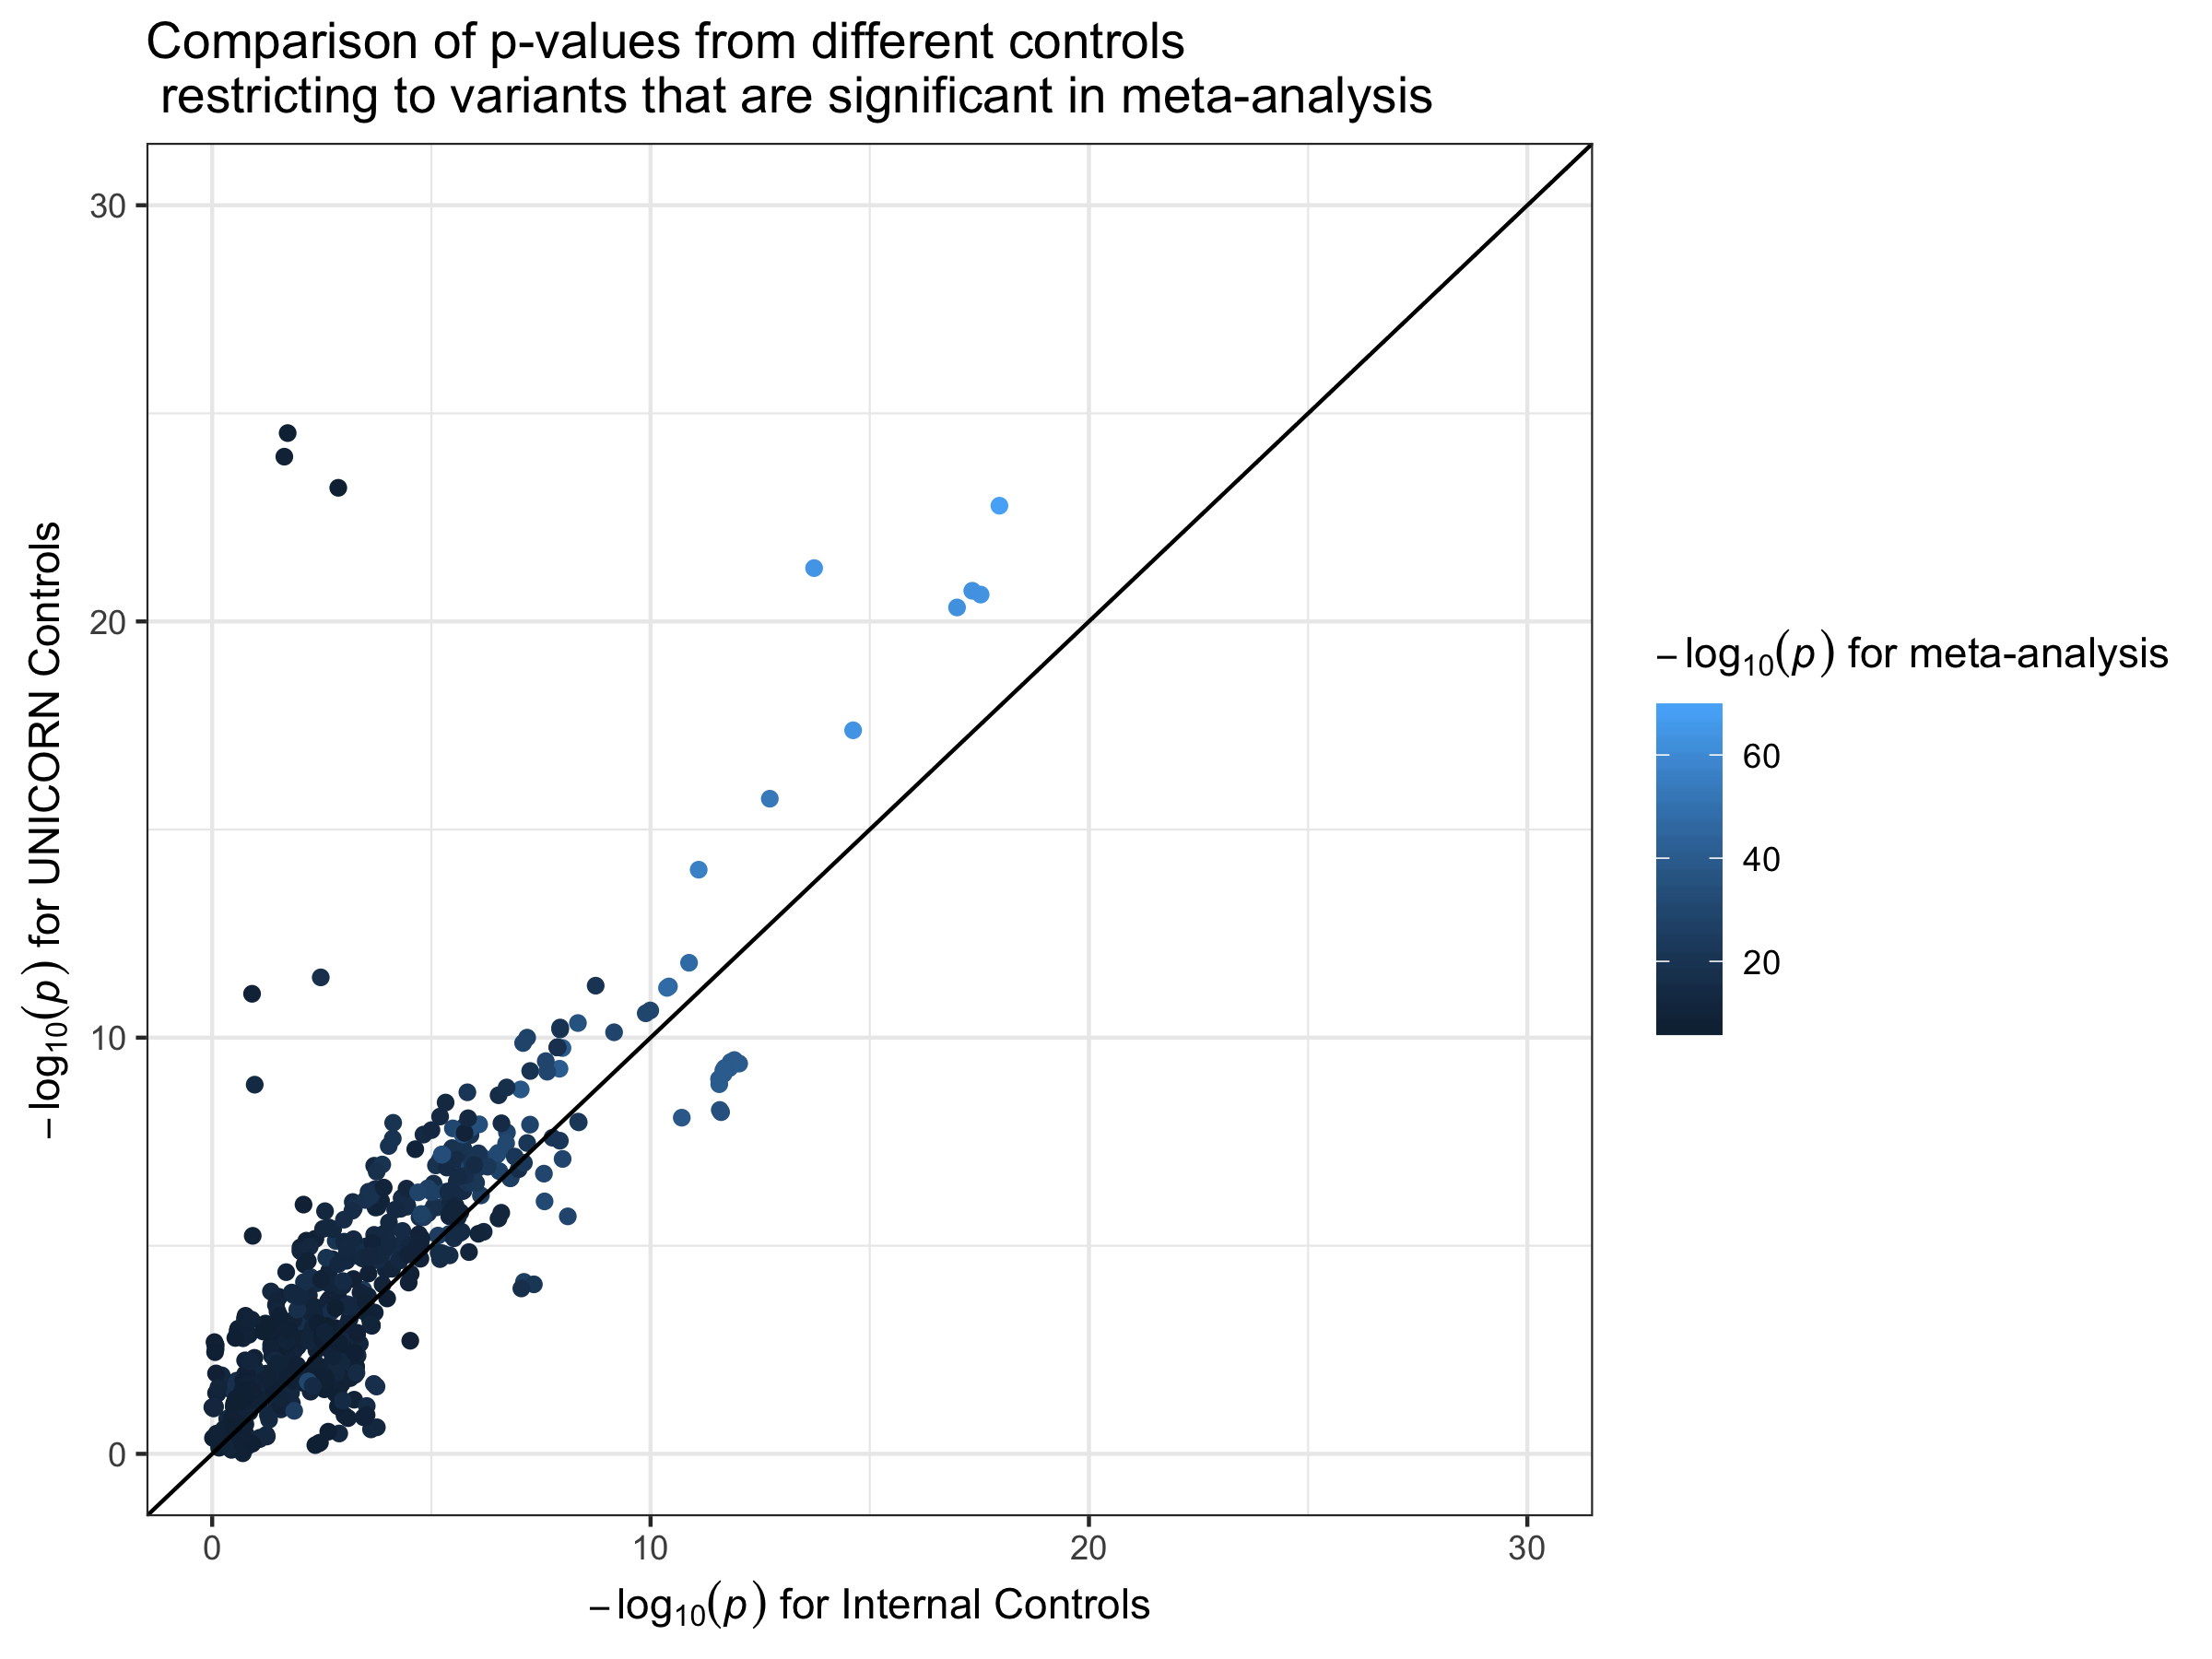
\includegraphics[width=0.49\textwidth]{qc/pvalues_significant.png}
    \caption{Comparison of p-values}
    \label{fig:pvalues}
\end{figure}


\section{A statistical framework for GWAS without direct accessing external controls}

Here we are demonstrating that we can make use of the harmonized external genotyping controls to boost power in GWAS studies. The general idea is that if the controls are numerous than cases, they typically span a large range of ancestries than cases, and it should be possible to find one or more controls similar to case.  Meanwhile, we can view control samples as mixtures of relatively homogeneous populations. Based on hierachical clustering with PCA, the control set is used to learn a decision tree clustering samples with similar ancestry. Cases are assigned to clusters using the same decision rules, without any data exchanging in hands. After creating matched strata based on ancestry, we use statistical methods tailored for finely-stratified data to perform association testing between disease outcome Y and test locus genotype G. Here, we use the Cochran-Mantel-Haenszel to test for disease-SNP association in the finely stratified data.  
\subsection{Inferring homogeneous populations (Tree-Building)}
This section describes how we infer homogeneous populations among controls. The homogeneous populations is defined based on the following criteria: 1) all eigenvalues capture noises and 2) sample size is too low that the estimated eigenvectors cannot well calibrate the true eigenvectors. \\
 %% How to justify why we don't wanna use the eigenstrat to detect number of population structures in the data and why we can use the following test for detecting n spikes
A test for population structure is based on a theoretical result that the null eigenvalues in the tail follow pattern of $eigenvalue_i = \beta \times i^{2/3} + \epsilon$, where i is the index of eigenvalues, $\beta$ is the scalar we're not interested in, and $\epsilon$ is the random noise term. Therefore, to test population structure, we fit a regression line without the largest eigenvalue, and test whether the largest eigenvalue is an outlier of the regression line. 

We use an iterative clustering algorithm to form hierarchical groups of mutually exclusive homogeneous clusters. In details, first of all, we run eigenvalue decomposition and any samples with first 10 PCs lying outside 5 standard deviation away from its mean are excluded. Then number of eigenvectors that captured ancestry ($n_{\text{spike}}$)are calculated using the test defined above. We use Gaussian mixture clustering to form $n_{\text{spike}} + 1$ sub-clusters with the first $n_{\text{spike}}$ principal components as features for clustering. Samples with mahalanobis distance greater than certain threshold to any cluster centers are considered to be outliers in ancestral space, and thus excluded. For each sub-cluster, we repeat those steps until the stopping criteria is met. The stopping criteria is defined to be $n_{\text{spike}} $ equals to zero or number of samples less than 200. 


\subsection{Estimating cases' ancestral origin}

Each case is projected onto the ancestral space with the PC loadings and control minor allele frequencies. We corrected the shrinkage with the software hdpca, and applied the same decision rule for determining the ancestral membership for cases. Mahalanobis distance was also applied to identify samples that are outliers in ancestry space. 

\subsection{Inference}
CMH test.

\subsection{Results}

\subsubsection{Simulation}
\begin{enumerate}
\item \emph{Unstratified phenotype}: among 22,000 samples, 20\% samples are randomly assigned to be cases while the rest are assigned to be controls. 
\item \emph{Stratified phenotype:} we simulated continuous phenotype constructed from PC1 plus some random noise and applied the liability threshold model to convert continuous phenotype to binary phenotype. Similar to unstratified phenotype setting, among 22,000 samples, 18.000 samples are assigned to be controls and 4,000 are assigned to be cases. 
\end{enumerate}
We run 10 simulations in each setting and reported the median lambda GC, and $N_{\mbox{effective}}$ calculated from UNICORN and standard GWAS. Different mahalanobis distance thresholds ranging from 3.5 to 5.0 for tree building and cases projecting were applied. 

\subsubsection{Real Data} We tested the performance of the UNICORN statistical framework with 6 IBD Crohn's collection. 


\begin{center}
{\color{red} FIG12: Manhattan plot and QQ plot}\\
{\color{red} FIG13: Plot for characterizing residual stratification}\\
{\color{red} TABLE6: Median lambda GC and $N_{\mbox{effective}}$}
\end{center}

\printbibliography


\end{document}
